\documentclass[man, floatsintext]{apa6}
% floatsintext so that figures show up where we want them to (https://www.tug.org/pracjourn/2012-1/beitzel/beitzel.pdf)
\usepackage{lipsum}
\usepackage{amsmath}

\usepackage[american]{babel}
\usepackage{ulem}
\usepackage{graphicx}
\usepackage{csquotes}
\usepackage{hyperref}
\usepackage[style=apa,sortcites=true,sorting=nyt,backend=biber]{biblatex}
\DeclareLanguageMapping{american}{american-apa}
\addbibresource{project1.bib}

\title{Analysis of Customer Churn at Telco}

\shorttitle{Customer Churn}

\author{Pedro Uria, Sean Pili, and Zachary Buckley}

\affiliation{George Washington University}

\begin{document}
\maketitle

\section{Introduction and Background Research}
\paragraph{Churn Rate}

In business, churn rate is the percentage of a company's customers that terminate their relationship with that company during a given time period. In the telecommunications industry, churn rates can be especially high because there is fierce competition and the market is saturated. In fact, in a study of factors that explain customer churn rates for an unidentified Indian telecommunications company, the authors mention that ``worldwide, the rate of customer churn in the telecom service industry ranges from 20 percent to 40 percent per year'' (\cite[p.~224]{Asamoah_2018}). If a company loses 20-40 percent of its existing customer base every year, that can have a significant negative effect on its revenue, regardless of how many new customers they obtain.  Consequently, many companies in saturated markets keep track of monthly, quarterly, and yearly churn rates in an attempt to identify defining characteristics of customers who churn, in order to predict and eventually reduce their customer churn rate.

Much of the scientific research on reducing customer churn across all industry verticals involves using logistic regression or other classification methods to predict which customers will churn in a given time period (typically monthly.) Common features used as classifiers include different aspects of customer purchasing behavior; their tenure (the length of a customer's relationship with a company), their account charges, and the frequency of their transactions (depending on the type of business). In 2015, Jarvis and Zorn ran an analysis on consumer data from an Australian internet DVD rental firm. The study attempted to determine if adding features measuring ``customer satisfaction, attitude and commitment'' to churn classification models, initially based on the aforementioned aspects of customer purchasing behavior, would increase their prediction accuracy (\maskciteyear[p.~1]{Jarvis_2015}). Interestingly, they found that ``the most significant predictor of churn in [customer purchasing habits, satisfaction and attitude] was a measure of uncertainty and commitment: the number of times a customer changed their subscription plan''(\maskCite[p.~1]{Jarvis_2015}). The study did not elaborate on how the customers changed their plans. That is to say, did the customers add or subtract services from their plans or alter other aspects of their plans entirely?

\hspace{0.5mm}

\paragraph{Telco Dataset}

We then searched for churn data on which we could test for the significance of relationships between customer purchasing behavior and a measure of customer commitment. The Telco Customer Churn Dataset we will be using throughout this paper contains information about the customers from an unidentified telecommunications company. The data was uploaded to \href{https://www.kaggle.com/blastchar/telco-customer-churn}{Kaggle} by a user named blastchar (\maskciteyear{blastchar_2018}). The dataset originates from a sample dataset provided by IBM for exploring the capabilities of their Watson Analytics services. IBM uses the data in a walkthrough of building a model for predicting whether a customer will leave the company, with the explicit goal of creating better customer retention programs. \cite{ibm_telco_2015} We were unable to determine conclusively if the Telco Dataset we are interested in for this paper was based on data from a real telecommunications company, or if the data was synthetically generated for the purposes of demonstrating the Watson Analytics system's capabilities.

That dataset consists of a snapshot of a (possibly fake) telecom company's customer database collected on a given month. It consists of 21 variables for 7043 customers, 26\% of which churned in the month prior to the data being collected. The variables cover a wide range of customer information including:
\begin{itemize}
  \item Demographics (\texttt{gender, dependents, ...})
  \item Service Options (\texttt{PhoneService, InternetService, ...})
  \item Billing (\texttt{PaperlessBilling, PaymentMethod, ...})
  \item Purchasing Behavior (\texttt{MonthlyCharges, tenure, ...})
\end{itemize}

\section{Research Question, Hypotheses, and Methods}

The variables that we will focus on are ContractType, MonthlyCharges, and Tenure in their relation to Churn, because they are the most similar to what the researchers were discussing.

\texttt{ContractType} is a categorical value that tells us whether a customer has a monthly, 1-year or 2-year contract. We'll use contract type as a proxy for a customers level of commitment to the company.

\texttt{MonthlyCharges} is a continuous variable that gives the amount of dollars charged to a customer in the previous month.

\texttt{Tenure} is a continuous variable that gives the number of months the customer has been with the company.

Both monthly charges, and tenure will be used as a proxy for purchasing behavior.

\hspace{0.5mm}

\paragraph{Research Question}

Are there significant relationships between a customer's \texttt{ContractType}, \texttt{MonthlyCharges}, \texttt{Tenure}, and whether they will Churn?

\hspace{0.5mm}

\paragraph{Hypotheses}

\begin{itemize}
\item \texttt{ContractType} $\begin{cases}
H_0: \texttt{Churn} \hspace{1mm} \text{and}  \hspace{1mm} \texttt{ContractType} \hspace{1mm} \text{are independent} \\
H_1: \texttt{Churn} \hspace{1mm} \text{and} \hspace{1mm} \texttt{ContractType} \hspace{1mm} \text{are not independent}
\end{cases}$
\item \texttt{MonthlyCharges} $\begin{cases}
H_0: \mu_{\text{Churn}} = \mu_{\text{NotChurn}} \\
H_1: \mu_{\text{Churn}} > \mu_{\text{NotChurn}}
\end{cases}$
\item \texttt{Tenure} $\begin{cases}
H_0: \mu_{\text{Churn}} = \mu_{\text{NotChurn}} \\
H_1: \mu_{\text{Churn}} < \mu_{\text{NotChurn}}
\end{cases}$
\end{itemize}

\subsection{Methods}

\paragraph{ContractType}
Since \texttt{Churn}, and \texttt{ContractType} are both categorical variables, the levels of each are mutually exclusive, and there are at least 5 customers that fall into each permutation of the variables levels, we can use a $\chi^2$-test.

\paragraph{MonthlyCharges and Tenure}
 Since \texttt{MonthlyCharges} and \texttt{tenure} are continuous variables we'll use t-tests to evaluate the null hypotheses. ($\mu_{\text{Churn}} = \mu_{\text{NotChurn}}$)

\section{Findings (EDA and Model Results)}

\hspace{0.5mm}

\noindent\begin{minipage}{0.54\textwidth}
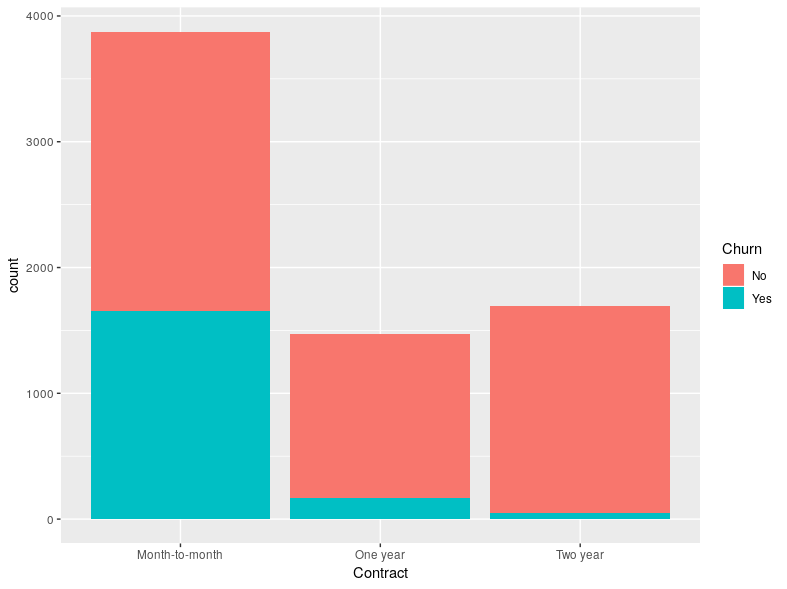
\includegraphics[width = \linewidth, height = 72mm]{CountvsContractTypebyChurn}
\end{minipage}
\hfill
\begin{minipage}{0.42\textwidth}
  \paragraph{Contract Type}
  We use the stacked bar plot to the left to visually determine if \texttt{Churn} and \texttt{ContractType} might be independent. There appears to be a clear difference in the ratio of the frequencies of churning and non-churning customers across each contract type. We can check if this difference is statistically significant by running a $\chi^2$-test.

\end{minipage}

\hspace{0.5mm}

The results of this $\chi^2$-test, give us a test statistic of $\chi^2 = 1184.6$ and $p < 2.2 \cdot 10^{-16}$. Thus we reject the null hypothesis at the $5 \%$ level of significance and say that \texttt{ContractType} and \texttt{Churn} are related.

\hspace{0.5mm}

\noindent\begin{minipage}{0.54\textwidth}
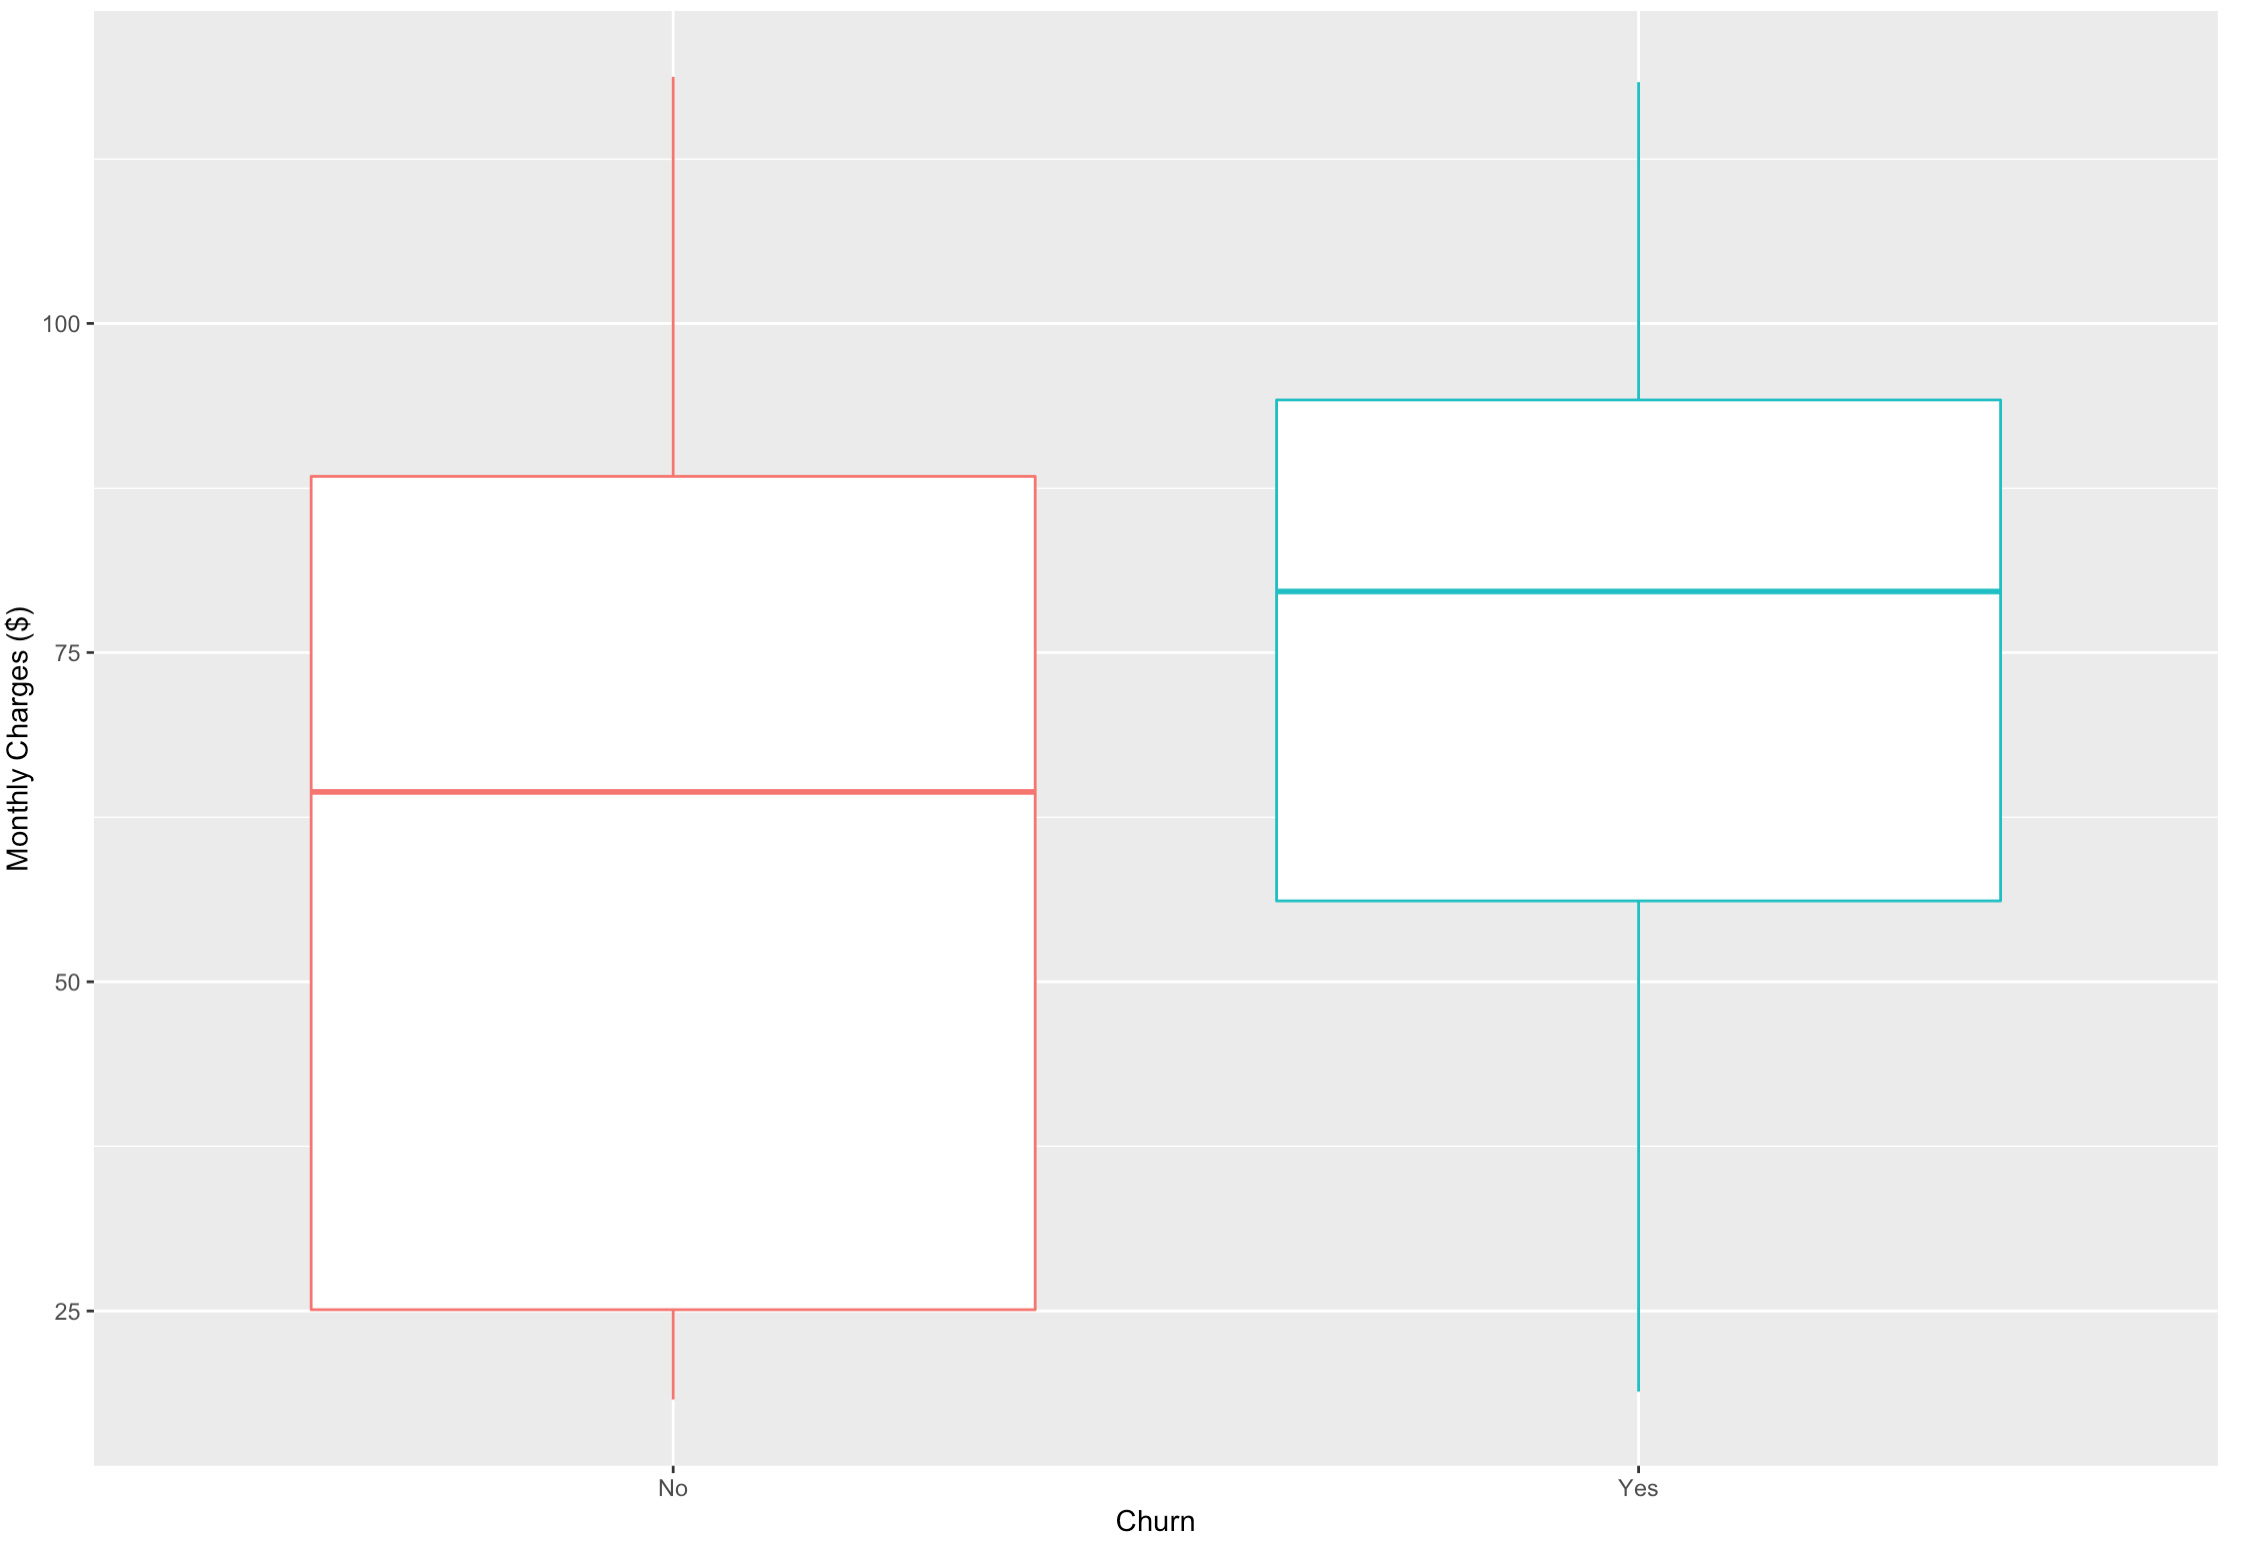
\includegraphics[width = \linewidth, height = 64mm]{boxplot_MonthlyChargesvsChurn}
\end{minipage}
\hfill
\begin{minipage}{0.43\textwidth}
   \paragraph{MonthlyCharges}
   By looking at the boxplot of \texttt{MonthlyCharges} grouped by \texttt{Churn}, we realize that the median of monthly charges for customers who churned appears to be greater than that of the customers who have not churned, which is why we decided to conduct a one-sided $t$-test.\\
\end{minipage}

\noindent\begin{minipage}{0.54\textwidth}
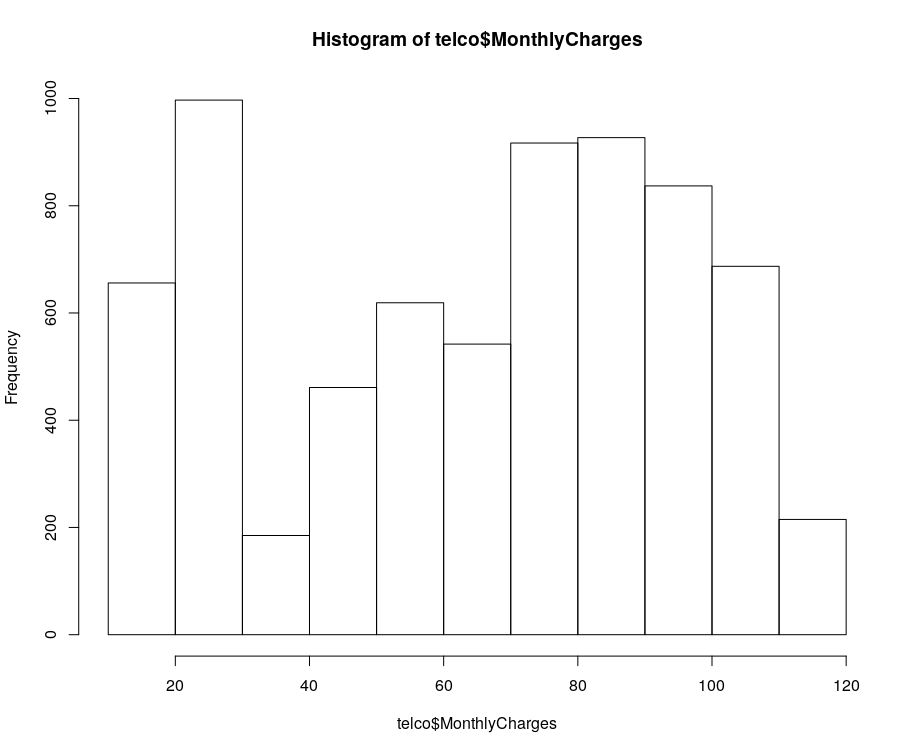
\includegraphics[width = \linewidth, height = 72mm]{hist_MonthlyCharges}
\end{minipage}
\hfill
\begin{minipage}{0.43\textwidth} Notice how the distribution of the monthly charges is not normally shaped. However, what we are comparing are means, and the Central Limit Theorem assures us that these means will follow a normal distribution for a large enough sample size, which enables us to perform the one-sided $t$-test. As in our case, we have 1869 churning customers, and 5174 non-churning customers.
\end{minipage}

\hspace{0.5mm}

After re-inspecting the boxplots above we can see how the variances of both groups are clearly different, and because of this we can't use a Student's $t$-test to test $\mu_{\text{Churn}} = \mu_{\text{NotChurn}}$. Instead, we will use a Welch's $t$-test, which does not assume equality of variances.

Upon running this test using R, we get a $p$-value $< 2.2 \cdot 10^{-16}$, which leads us to reject $H_0$ at the  $\alpha = 0.05$ level of significance, and consider our alternative hypothesis: customers who churned are paying more on average than customers who have not churned.

\newpage

\paragraph{Tenure}

By looking at the boxplot of \texttt{Tenure} grouped by \texttt{Churn} below, we notice that the median \texttt{Tenure} of churning customers is roughly 1/4 the median \texttt{Tenure} of the non-churning customers (10 to roughly 38 months respectively), which is why we decided to conduct a one-sided $t$-test.

After further inspection, we can see how the variances of both groups are clearly different, and because of this we can't use a Student's $t$-test to test $\mu_{\text{Churn}} = \mu_{\text{NotChurn}}$. Instead, we will use a Welch's $t$-test, which does not assume equality of variances.

Notice that \texttt{Tenure} is not normally distributed in the histogram below. However, as we mentioned before, t-tests are robust to non-normality given that our sample sizes are large enough.

\hspace{0.5mm}

\noindent\begin{minipage}{0.485\textwidth}
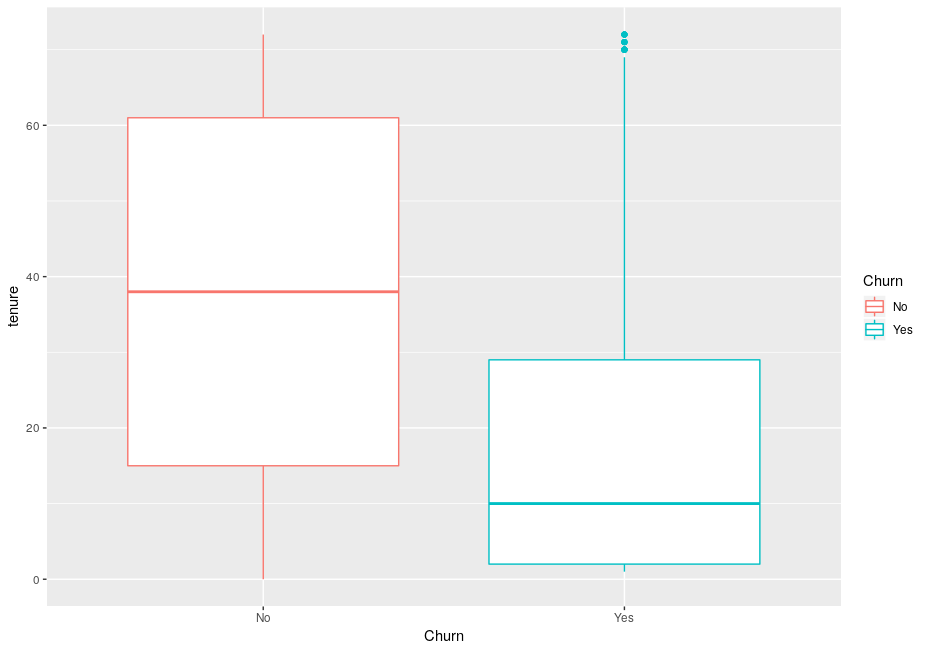
\includegraphics[width = \linewidth]{boxplot_tenurebyChurn}
\end{minipage}
\hfill
\begin{minipage}{0.5\textwidth}
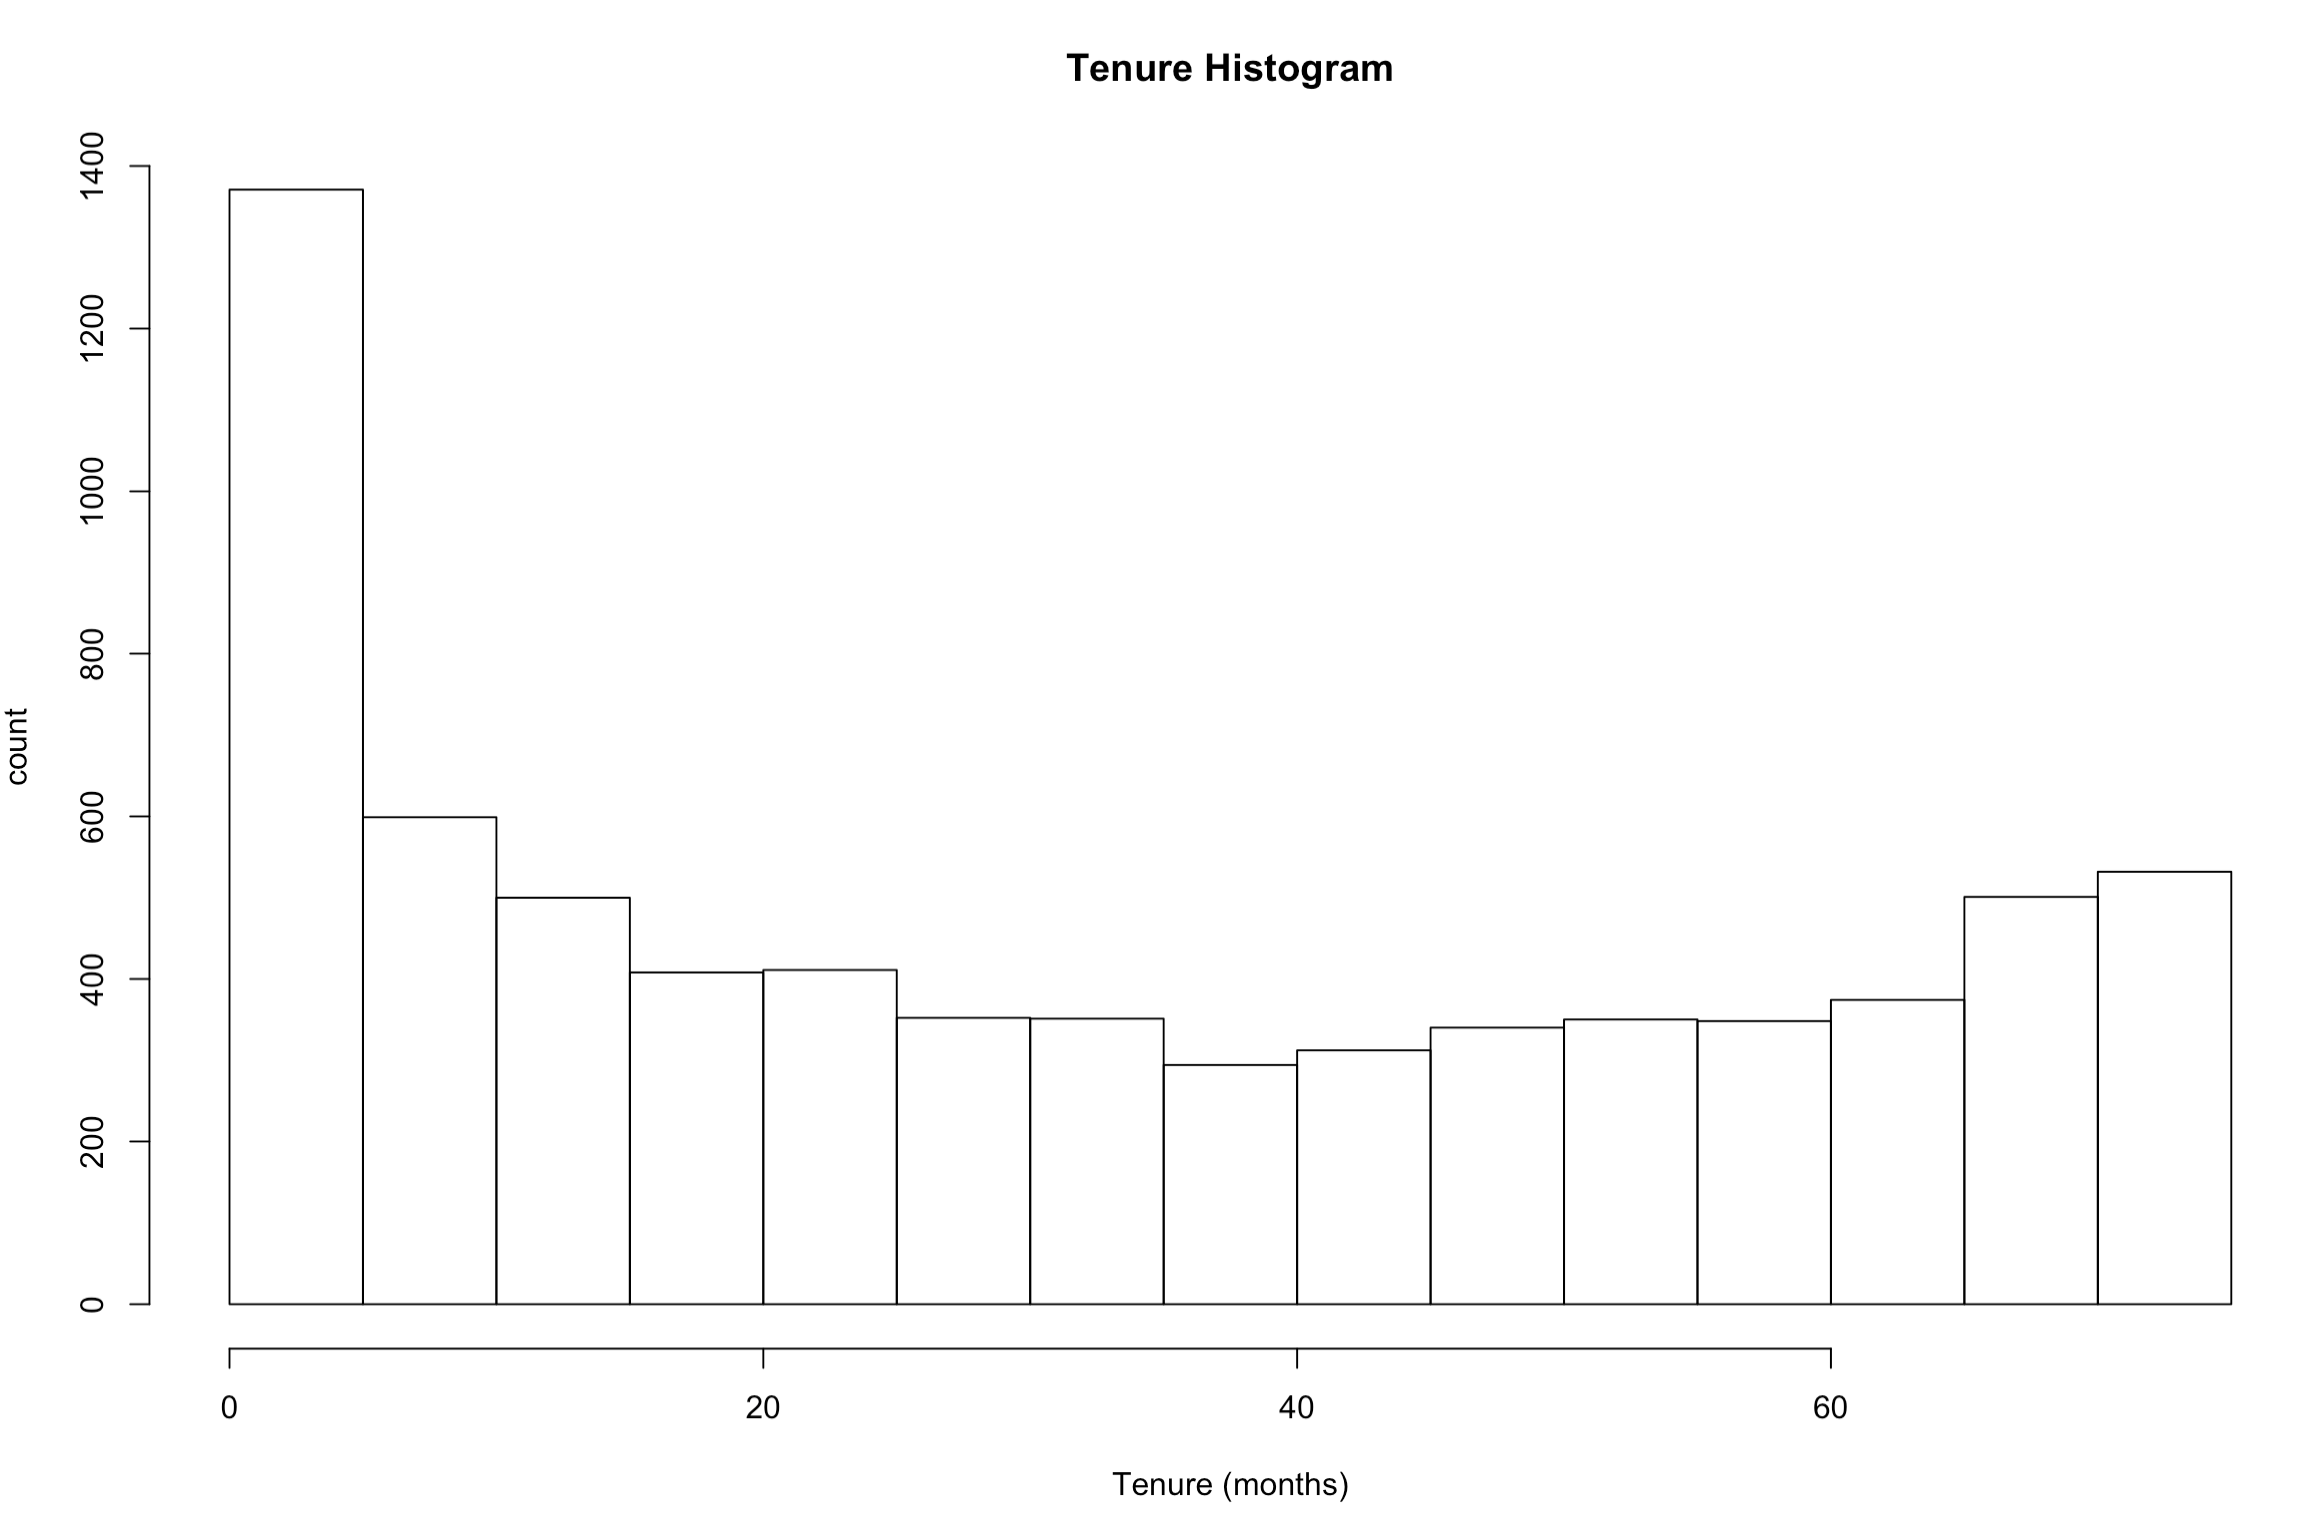
\includegraphics[width = \linewidth]{histogram_Tenure}
\end{minipage}

\hspace{0.5mm}

In this case, we also get a very small $p$-value (again $< 2.2 \cdot 10^{-16}$), so we reject the null hypothesis that $H_0: \mu_{\text{Churn}} = \mu_{\text{NotChurn}}$ at the $\alpha = 0.05$ level of significance and consider our alternative hypothesis: customers who haven't churned have been with the company longer on average.

\section{Conclusions}

By performing a combination of Explanatory Data Analysis and Hypothesis Testing, we have come to the conclusion that, as we expected, there are significant relationships between \texttt{Churn} and the three variables \texttt{ContractType}, \texttt{MonthlyCharges} and \texttt{Tenure}.

In particular, the dependence between \texttt{ContractType} and \texttt{Churn} has been tested by a $\chi^2$-test. We have also seen, by running one-tailed $t$-tests, that the mean of \texttt{MonthlyCharges} is greater for customers who churned, and that the mean of \texttt{Tenure} is greater for customers who haven't churned.

Therefore it makes sense that researchers studying churn rates typically would include a customer's tenure, monthly charges, and a proxy for customer commitment in a logistic regression or classification model, as our literature review suggests.

\newpage
\printbibliography
\end{document}
